\documentclass[12pt]{report}

\usepackage{amsmath}
\usepackage{graphicx}
\usepackage{listings}
\usepackage{hyperref}
\usepackage{algorithm2e}
\usepackage[a4paper, total={7in,9in}, headheight=14pt]{geometry}
\usepackage{minted}

\lstset{breaklines=true}
\lstset{language=C++,
        basicstyle=\ttfamily,
        stringstyle=\color{red},
        commentstyle=\color{green},
        breaklines=true,
        showstringspaces=false}

\title{Combined Report of Weeks 1 to 9}
\author{Ananth Krishna Kidambi, Guramrit Singh}
\begin{document}
    \maketitle
    \tableofcontents
    \chapter*{Week 9}
    \addcontentsline{toc}{chapter}{Week 9}
    \section*{Code Implementation}
    This week, we added support for infinite precision integers using the \texttt{gmp} library to the numerical evaluation part. Now, all functions take arguments (domain sizes) as unsigned integers and return \texttt{mpz\_class} objects (defined in the \texttt{gmpxx.h} header). 
	Besides this, we also removed Wolframscript simplification (since that was slow) and added a CLI option \texttt{--sizes} to specify the domain sizes on the command line. 
    \subsection*{Example}
    Consider the set of equations - 
    \begin{align*}
        f0(x0,x1)&=\sum_{x2=0}{x1}((-1)^{x1-x2}\cdot\\ & \binom{x1}{x2}\cdot \sum_{x3=0}{x0}[(-1)^{x0-x3}\cdot \binom{x0}{x3}\cdot f1(x2,x3))\\
        f1(x2,x3)&=\binom{x3}{0}\cdot f1(-1+x2,x3-0)+\binom{x3}{1}\cdot f1(-1+x2,x3-1)\\
        f1(0,x3)&=1\\
        f1(x2,0)&=1\\
    \end{align*}
    The corresponding code generated is - 
    \begin{minted}[tabsize=4,linenos]{cpp}
#include <iostream>
#include <string>
#include <vector>
#include <cmath>
#include <gmpxx.h>

class cache_elem{
public : 
	mpz_class n;
	cache_elem(mpz_class x) : n{x} {}
	cache_elem() : n{-1} {}
};

template <class T> T& get_elem(std::vector<T>& a, size_t n){
	if (n >= a.size()){
		a.resize(n+1);
	}
	return a.at(n);
}

mpz_class Binomial(unsigned int n, unsigned int r){
	mpz_t ans;
	mpz_init(ans);
	mpz_bin_uiui(ans, n, r);
	return mpz_class{ans};
}

mpz_class power(mpz_class x, unsigned int y){
	mpz_t ans;
	mpz_init(ans);
	mpz_pow_ui(ans, x.get_mpz_t(), y);
	return mpz_class{ans};
}

std::vector<cache_elem> f0_cache;
std::vector<std::vector<cache_elem>> f1_cache;

mpz_class f0(unsigned int x0);
mpz_class f1(unsigned int x1, unsigned int x2);
mpz_class f1_0x(unsigned int x2);
mpz_class f1_x0(unsigned int x1);

mpz_class f0(unsigned int x0){
	mpz_class& stored_val = get_elem(f0_cache, x0).n;
	if (stored_val != -1)
		return stored_val;
	if (x0 >= 0){
		mpz_class ret_val = ([x0](){mpz_class sum{0}; for (unsigned x1 = 0; x1 <= x0; x1++){ sum += (Binomial(x0,x1)*(power(-1,x0-x1)*([x0,x1](){mpz_class sum{0}; for (unsigned x2 = 0; x2 <= x0; x2++){ sum += (Binomial(x0,x2)*(power(-1,x0-x2)*f1(x1,x2)));} return sum;})()));} return sum;})();
		get_elem(f0_cache, x0).n = ret_val;
		return ret_val;
	}
	exit(1);
	return -1;
}
mpz_class f1(unsigned int x1, unsigned int x2){
	mpz_class& stored_val = get_elem(get_elem(f1_cache, x1), x2).n;
	if (stored_val != -1)
		return stored_val;
	if (x1 >= 1 && x2 >= 1){
		mpz_class ret_val = (Binomial(x2,0)*f1(x1-1,x2-0))+(Binomial(x2,1)*f1(x1-1,x2-1));
		get_elem(get_elem(f1_cache, x1), x2).n = ret_val;
		return ret_val;
	}
	else if (x1 == 0){
		return  f1_0x( x2);
	}
	else if (x2 == 0){
		return  f1_x0( x1);
	}
	exit(1);
	return -1;
}
mpz_class f1_0x(unsigned int x2){
	mpz_class& stored_val = get_elem(get_elem(f1_cache, 0), x2).n;
	if (stored_val != -1)
		return stored_val;
	if (x2 >= 0){
		mpz_class ret_val = 1;
		get_elem(get_elem(f1_cache, 0), x2).n = ret_val;
		return ret_val;
	}
	exit(1);
	return -1;
}
mpz_class f1_x0(unsigned int x1){
	mpz_class& stored_val = get_elem(get_elem(f1_cache, x1), 0).n;
	if (stored_val != -1)
		return stored_val;
	if (x1 >= 0){
		mpz_class ret_val = 1;
		get_elem(get_elem(f1_cache, x1), 0).n = ret_val;
		return ret_val;
	}
	exit(1);
	return -1;
}

int main(){
	std::cout << f0(2048) << std::endl;
}
    \end{minted}
    \chapter*{Week 8}
    \addcontentsline{toc}{chapter}{Week 8}
    \section*{Code Implementation}
    This week, the implementation of numerical evaluation was completed. This is done by converting the recursive equations into a \texttt{C++} program, which can then be compiled and executed to obtain numerical values. 

    The translation of a set of equations($E$) into \texttt{C++} works as follows - 
    \begin{enumerate}
        \item First, we create a cache for each function in $E$. For a function with name \texttt{func}, this cache is called \texttt{func\_cache}. This is implemented as a multi-dimensional vector containing objects of \texttt{class cahce\_elem} defined as shown in the example code. The default initialization of this object is to $-1$ which is useful for recognizing unevaluated cases.
        \item Next, we create a function definition for each lhs in $E$, including all functions and base cases. The signatures of these functions is decided as follows - a function call containing only variable arguments is named as the function itself, and ones with constants in their arguments are suffixed with a string that contains \texttt{'x'} at the $i$th place if the $i$th argument is variable and the $i$th argument if that argument is a constant. For example, $f(x1, x2, x3)$ is declared as \texttt{int f(int x1, int x2, int x3);} and $f(1, x2, x3)$ is declared as \texttt{int f\_1xx(int x2, int x3);} (the constant arguments are removed from the signature).
        \item The rhs of each equation in $E$ is used to define the body of the equation corresponding to the lhs of that equation. The function body (for a function \texttt{func} corresponding to equation $e$) is formed as follows-
        \begin{enumerate}
            \item First, we check if the evaluation is already present in the cache. If so, then we return the cache element. The cache accesses are done using the \texttt{get\_elem} function(definition given in the example), which resizes the cache if the accessed index is out of range. 
            \item If the element is absent, then we decide if the arguments corresponding to $e$ or one of the functions corresponding to the base cases, based on the value of the arguments. If it corresponds to the base cases, then we directly call the base case function and return its value. Else, we evaluate the value using the rhs, store the evaluated value in the cache and return the evaluated value. Note that in this step, we only call the base case function with one more constant argument that \texttt{func}. For example, \texttt{f0(x, y)} would call \texttt{f0\_0x(y)} if \texttt{x == 0} and \texttt{f0\_x0(x)} if \texttt{y == 0}.
            \item In order to translate the rhs, we do the following changes-
            \begin{itemize}
                \item \verb|a^b| is converted to \texttt{power(a,b)}.
                \item \texttt{Sum[exp, x, a, b]} = ($\sum_{x=a}^{b}exp$) is converted to -\\
                \begin{lstlisting}
([y,z,...](){
    int sum{0};
    for(int x{a}; x <= b; x++)
        sum += exp;
    return sum;
})()
                \end{lstlisting}
                where y, z, ... are the free variables present in \texttt{exp}.
            \end{itemize} 
        \end{enumerate}
    \end{enumerate}
    
    \subsection*{Example}
    Consider the set of equations - 
    \begin{align*}
        f0(x0,x1)&=\sum_{x2=0}{x1}((-1)^(x1-x2)\cdot\\ & Binomial(x1,x2)\cdot \sum_{x3=0}{x0}[(-1)^(x0-x3)\cdot Binomial(x0,x3)\cdot f1(x2,x3))\\
        f1[x2,x3]&=Binomial(x3,0)\cdot f1(-1+x2,x3-0)+Binomial(x3,1)\cdot f1[-1+x2,x3-1]\\
        f1[0,x3]&=1\\
        f1[x2,0]&=1\\
    \end{align*}
    The corresponding code generated is - 
    \begin{minted}[tabsize=4,linenos]{cpp}
#include <iostream>
#include <string>
#include <vector>
#include <cmath>

class cache_elem{
public : 
	int n;
	cache_elem(int x) : n{x} {}
	cache_elem() : n{-1} {}
};

template <class T> T& get_elem(std::vector<T>& a, size_t n){
	if (n >= a.size()){
		a.resize(n+1);
	}
	return a.at(n);
}

int Binomial(int n, int r){
	return round(std::tgamma(n+1)/(std::tgamma(r+1)*std::tgamma(n-r+1)));
}

int power(int x, int y){
	return round(pow(x, y));
}

std::vector<std::vector<cache_elem>> f0_cache;
std::vector<std::vector<cache_elem>> f1_cache;

int f0(int x0, int x1);
int f1(int x2, int x3);
int f1_0x(int x3);
int f1_x0(int x2);

int f0(int x0, int x1){
	int stored_val = get_elem(get_elem(f0_cache, x0), x1).n;
	if (stored_val != -1)
		return stored_val;
	if (x0 >= 0 && x1 >= 0){
		int ret_val = ([x0,x1](){int sum{0}; for (unsigned x2 = 0; x2 <= x1; x2++){ sum += ((power(-1,x1-x2)*Binomial(x1,x2))*([x0,x1,x2](){int sum{0}; for (unsigned x3 = 0; x3 <= x0; x3++){ sum += ((power(-1,x0-x3)*Binomial(x0,x3))*f1(x2,x3));} return sum;})());} return sum;})();
		get_elem(get_elem(f0_cache, x0), x1).n = ret_val;
		return ret_val;
	}
	return -1;
}
int f1(int x2, int x3){
	int stored_val = get_elem(get_elem(f1_cache, x2), x3).n;
	if (stored_val != -1)
		return stored_val;
	if (x2 >= 1 && x3 >= 1){
		int ret_val = (Binomial(x3,0)*f1(-1+x2,x3-0))+(Binomial(x3,1)*f1(-1+x2,x3-1));
		get_elem(get_elem(f1_cache, x2), x3).n = ret_val;
		return ret_val;
	}
	else if (x2 == 0){
		return  f1_0x( x3);
	}
	else if (x3 == 0){
		return  f1_x0( x2);
	}
	return -1;
}
int f1_0x(int x3){
	int stored_val = get_elem(get_elem(f1_cache, 0), x3).n;
	if (stored_val != -1)
		return stored_val;
	if (x3 >= 0){
		int ret_val = 1;
		get_elem(get_elem(f1_cache, 0), x3).n = ret_val;
		return ret_val;
	}
	return -1;
}
int f1_x0(int x2){
	int stored_val = get_elem(get_elem(f1_cache, x2), 0).n;
	if (stored_val != -1)
		return stored_val;
	if (x2 >= 0){
		int ret_val = 1;
		get_elem(get_elem(f1_cache, x2), 0).n = ret_val;
		return ret_val;
	}
	return -1;
}

int main(){
	std::cout << f0(3,3) << std::endl;
}
    \end{minted}
    \chapter*{Week 7}
    \addcontentsline{toc}{chapter}{Week 7}
    \section*{Code Implementation}
    The target is to generate C++ code that can evaluate numerical values of the model counts based on the equations generated by Crane. 

    There are two ways to do the same-

    \begin{enumerate}
        \item Generate C++ code by traversing the FCG, similar to what is done in \texttt{OutputVisitor.scala}.
        \item Parse the equations generated by crane after simplifying in wolfram and then generate C++ code.
    \end{enumerate}

    The problem with the first approach is that while generating base cases, the subsequent calls for crane do not necessarily have the same meanings for the function arguments and the functions.

    For example, if \texttt{f1[x0, x1, x2]} represents the model count of a constrained formula F, where f1 is an auxilliary formula and $x0 = |A|, x1 = |B|, x2 = |C|$, ($A,B,C$ are domains) and we want to evaluate \texttt{f1[0, x1, x2]}($|A| = 0$), then crane may return the required model count as \texttt{f0[x0, x1]}, where $x0 = |B|, x1 = |C|$. We'll need to translate this to \texttt{f1[0,x1,x2]}, which has already been implemented in \texttt{Basecases.scala}.

    Also, the second approach can be done in linear time in the length of the formula using the \href{https://en.wikipedia.org/wiki/Shunting_yard_algorithm#:~:text=In%20computer%20science%2C%20the%20shunting,abstract%20syntax%20tree%20(AST).}{Shunting Yard Algorithm}.

    Hence, we are implementing the second approach (have already implemented the parser).
    \chapter*{Week 6}
    \addcontentsline{toc}{chapter}{Week 6}
    \section*{Slight Change in Base Case Evaluation Idea}
    The previous method of base case evaluation on setting a domain to size 0 or 1 had the following error - in case a domain size was set to 0, it assumed that those predicates which were deleted from the clauses could take any truth value over the entire domain and the rest were fully covered by the remaining clauses. 
    
    For example, consider the constrained CNF formula - 
    \begin{align}
        \forall x \in \Delta \forall y, z \in \Gamma &: P(x) \lor Q(y, z) \\
        \forall y \in \Gamma^\top &: Q(y, z)
    \end{align}
    In this case, if we set $|\Delta|$ to $0$, then based on the previous idea, the new set of clauses would be 
    \begin{equation}
        \forall y, z \in \Gamma^\top : Q(y, z)
    \end{equation}
    and the set of removed predicates is $\phi$, and hence the model count returned would be $1$. However, the actual model count shoud be $2^{|\Gamma|^2 - |\Gamma^\top|^2}$.

    There are 2 ideas which we could think of to solve this - 
    \begin{enumerate}
        \item \textit{(Currently, we have implemented this)} Convert the clauses having universal quantification over the null domain to tautology clauses, hence retaining all the predicates which don't have an argument belonging to the null domain. For example, we would convert the above mentioned CNF formula to 
        \begin{align}
            \forall y, z \in \Gamma &: Q(y, z) \lor \neg Q(y, z) \\
            \forall y, z \in \Gamma^\top &: Q(y, z)
        \end{align}
        The model count returned by this will also consider the truth value of Q over $y \not \in \Gamma^\top$ or $z \not \in \Gamma^\top$.   
        \item We find the domain size over which the predicate has not been defined by the clauses and multiply the required factor. For example, in the above example, the multiplier would be $2^{|\Gamma|^2 - |\Gamma^\top|^2}$ and the simplified set of clauses would be 
        \begin{equation}
            \forall y, z \in \Gamma^\top : Q(y, z)
        \end{equation}
        which has a model count of $1$. Hence, the obtained value of model count would be $2^{|\Gamma|^2 - |\Gamma^\top|^2} \times 1$.
    \end{enumerate} 

    \chapter*{Detailed Summary of Algorithms}
    \addcontentsline{toc}{chapter}{Detailed Summary of Algorithms}

    \section*{Algorithm to Find a Sufficient Set of Base Cases}
    The pseudo-code of the algorithm is given below-

    \begin{algorithm}[H]
        \SetAlgoLined
        \caption{Algorithm For Sufficient Base Cases}
        \KwIn{dependencies}
        \KwOut{base\_cases}
        
        % Algorithm steps
        base\_cases $\leftarrow$ Set()

        \ForEach{dependency $\in$ dependencies}{
            \ForEach{elem $\in$ dependency.value}{
                \If{dependency.key.func\_name = elem.func\_name}{
                    \ForEach{arg $\in$ elem.args}{
                        \tcp{eg : lim is 2 for the arg (x-3)}
                        lim $\leftarrow$ arg.const\_subtracted - 1 \\
                        \For{l $\in$ 0 to lim}{
                            \tcp{eg : for dependency.key = f(x,y), arg = x and l = 0, add f(0, y) to base\_cases}
                            base\_cases += dependency.key.substitute\_arg(arg\_var, l)
                        }
                    }
                }
                \Else{
                    \ForEach{arg $\in$ elem.args}{
                        \tcp{eg : lim is 2 for the arg (x-3)}
                        lim $\leftarrow$ arg.const\_subtracted - 1 \\
                        \For{l $\in$ 0 to lim}{
                            \tcp{eg : for dependency.key = f(x,y), arg = x and l = 0, add f(0, y) to base\_cases}
                            base\_cases += dependency.key.substitute\_arg(arg, l)\\
                            \tcp{signature for f(x-1, y-2) is f(x,y)}
                            base\_cases += elem.signature.substitute\_arg(arg, l)
                        }
                    }
                }
            }
        }
    \end{algorithm}

    Here, \texttt{dependencies} maps the function call on the lhs of each equation to the set of function calls on the rhs of the equation. For example, for the equations 
    \begin{equation*}
        f(m, n) = g(m-1, n) + f(m-2, n-1) 
    \end{equation*}
    \begin{equation*}
        g(m, n) = f(m-1, n-2) + g(m-1, n-1)
    \end{equation*}
    the dependencies are -
    \begin{equation*}
        f(m,n) \mapsto \{g(m-1,n), f(m-2, n-1)\}
    \end{equation*}
    \begin{equation*}
        g(m, n) \mapsto \{f(m-1, n-2), g(m-1, n-1)\}
    \end{equation*}

    \section*{Algorithm to Transform CNF Based on Domain Sizes}

    The pseudo code is given below-
    \begin{algorithm}
        \SetAlgoLined
        \caption{Algorithm For Transforming CNF Based on Domain Sizes}
        \KwIn{cnf, dom, dom\_size}
        \KwOut{transformed\_cnf, multiplier}
        removed\_predicates $\leftarrow$ Set()
        retained\_predicates $\leftarrow$ Set()
        \If{dom\_size = 0}{
            \ForEach{clause $\in$ cnf}{
                \If{dom $\in$ clause.domains}{
                    removed\_predicates += clause.predicates
                }
                \Else{
                    retained\_predicates += clause.predicates
                    transformed\_cnf += clause
                }
            }
            removed\_predicates = removed\_predicates $\setminus$ retained\_predicates
            \ForEach{pred $\in$ removed\_predicates}{
                multiplier *= $2^{(pred.domain\_sizes.join("*"))}$
            }
        }
        \ElseIf{dom\_size = 1}{
            const $\leftarrow$ newConst()
            \ForEach{clause $\in$ cnf}{
                transformed\_clause $\leftarrow$ clause
                \ForEach{v $\in$ clause.vars | v.domain = dom}{
                    transformed\_cnf $\leftarrow$ transformed\_clause.substituteVar(v, const)
                }
                transformed\_cnf += transformed\_clause
            }
        }
    \end{algorithm}

    We use Algorithm 2 to find the transformed cnf corresponding to each base case obtained using Algorithm 1 and call crane on the cnf to obtain the required base cases.

    \chapter*{Week 5}
    \addcontentsline{toc}{chapter}{Week 5}
    

    This week, we implemented the evaluation of basecases. The evaluation is done by simplifying the clauses and then using CRANE to find the basecases.
    \vspace*{0in}

    First, in the \texttt{SimplifyUsingWolfram} class, while traversing the graph to find the equations, we store 2 \texttt{Map} objects - \texttt{clause\_func\_map}(which stores the mapping from the function names to the formulae, whose model count they represent) and \texttt{var\_domain\_map}(which stores the mapping from the variable names to the domains whose sizes they represent).
    \vspace*{10px}

    Then, a particular domain is selected(using the algorithm described in previous reports) and the clauses are simplified. Then, CRANE is called on those clauses to evaluate the base cases using \texttt{WeightedCNF.SimplifyInWolfram}. After that, we change the function names and variable to make it consistent with the previous domain to variable mapping, and append these basecases to the set of equations.

    \section*{Issues With Wolfram}
    Wolfram is too slow when trying to expand after replacing Piecewise with Boole. For example, the code 
    \begin{lstlisting}
        Simplify[ Sum[Binomial[x0, x1] * (-1.0)^((x0 - x1)) * Sum[Binomial[x0, x2] * (-1.0)^((x0 - x2)) * Sum[Binomial[x2, x3] * Boole[0 <= x3 < 2], {x3, 0, x2}]^(x1), {x2, 0, x0}], {x1, 0, x0}]]
    \end{lstlisting}
    doesn't even simplify on using wolframscript.
    Even when the evaluation is done on the cloud, the engine times out after one minute. 
    We also tried some statergies mentioned \underline{\href{https://community.wolfram.com/groups/-/m/t/989124}{here}}, which didn't help. 

    \chapter*{Week 4}
    \addcontentsline{toc}{chapter}{Week 4}

    \section*{Code Implementation}
    The following steps were followed while finding the basecases-
    \begin{enumerate}
        \item Expand the summations in each equation - Here we expand the summations of the form: $\sum_{x=0}^{x1}<\textnormal{something}> \cdot [a \le x < b]$, or similar inequalities where x is bounded by constants and $a$ and $b$ are constants, by substituting the value of x from $a$ to $b-1$.
        For example, we replace $\sum_{x=0}^{x_1} {{x_1}\choose{x}} f(x_1-x)\cdot[0 \le x < 2]$ by ${{x_1}\choose{0}}f(x_1) + {{x_1}\choose{1}}f(x_1-1)$.
        \item Next, we find the dependencies of those functions that appear on the rhs of any equation. Consider, for example the following set of equations-
        \begin{align}
            f0(m, n) &= f1(m-1, n) + f2(m, n-1)\\
            f1(m, n) &= f1(m-1, n-1) \times f2(m-2, n-1)\\
            f2(m, n) &= 2 \times f1(m-3, n-1)
        \end{align}
        In this case, the dependencies computed are 
        \begin{align*}
            f1(m, n) &\rightarrow f1(m-1, n-1), f2(m, n-1)\\
            f2(m, n) &\rightarrow f1(m-3, n-1) 
        \end{align*}
        \item Now, based on idea II of the previous report, we find a domain that has only terms of the form $x-1$ appearing on the rhs of the dependencies. The base cases are then calculated by setting this domain size to 0. For the above example, $n$ is the selected domain, and not $m$ since there are $m-2$ and $m-3$ terms appearing in the arguments.
    \end{enumerate}
    \section*{Limitations of the current code}
    \begin{itemize}
        \item Ideally, we should calculate the base cases based on idea II of the previous report by finding the basecases upto max$(c1, c2, ...) - 1$. However, we are yet to implement code for finding the basecases for the non-null domain case.
    \end{itemize}

    \chapter*{Week 3}
    \addcontentsline{toc}{chapter}{Week 3}

    \section*{Ideas for finding which base cases are needed}
    \subsection*{Idea I}
    One idea is that, if the sizes of the domains are already given, we could make a dependency graph based on the recursive equations given and find the values of the nodes of the graph with no outgoing edges. For example if the equations are -
    \begin{equation*}
        f(m, n) = g(m-1, n) + f(m-2, n-1) 
    \end{equation*}
    \begin{equation*}
        g(m, n) = f(m-1, n-2) + g(m-1, n-1)
    \end{equation*}
    with $m = 4$ and $n = 3$, the graph would be- 
    \begin{figure}[h]
        \centering
        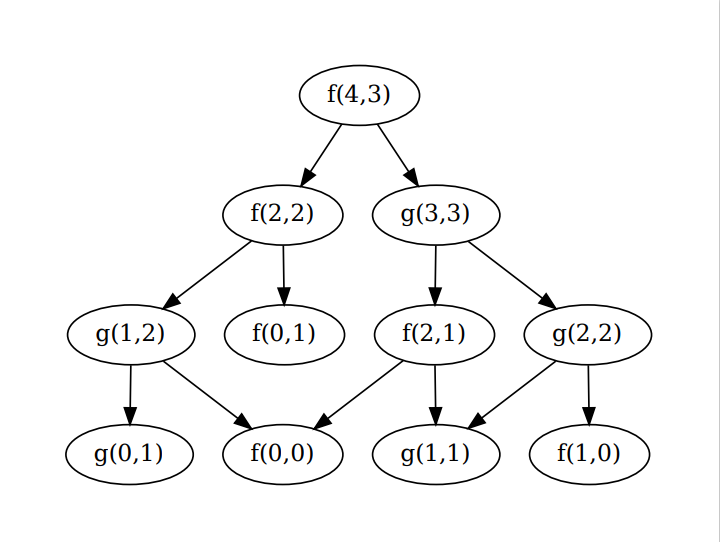
\includegraphics[width=8cm]{dep.png}
    \end{figure}
    In this case, the base cases evaluated will be $g(0,1), f(0,1), f(0, 0), g(1,1)$ and $f(1,0)$.
    \subsection*{Idea II}
    The goal is to find the sufficient set of base cases. We know that if say, on the rhs of all equations, the domain size appears as $m-c_1, m-c_2, \dots, m-c_k$, then finding $f(0, x_1, x_2, \dots)$, $f(1, x_1, x_2, \dots)$, $\dots f(m_0, x_1, x_2, \dots)$ for every function $f$, where $m_0 = \textnormal{max}(c_1, c_2, \dots c_k) - 1$ forms a sufficient set of base cases.
    Hence, in order to do the same efficiently, we can take that domain for which $m_0$ is the minimum, i.e. $argmin(\textnormal{max}(c_1, c_2, \dots c_k))$. 

    \section*{Finding the model counts for base cases}
    If a domain is set to $0$, the model count can be found by simplifying the universal and existential quantifiers over that domain, and then using crane. 
    
    However, if a domain is set to contain some non-empty number of elements, we can apply GDR over that domain and proceed with crane, substituting the known values of preveiously calculated model counts in the process. 

    \chapter*{Week 2}
    \addcontentsline{toc}{chapter}{Week 2}

    \begin{itemize}
        \item Read the Crane paper and the recursion part of the thesis by Paulius.
        \item Modified the wolfram simplification functions to incorporate binomial and indicator functions.
        \item Went through some parts of the codebase.
        \item No concrete idea found for finding base cases.
    \end{itemize}

    \chapter*{Week 1}
    \addcontentsline{toc}{chapter}{Week 1}

    \begin{itemize}
        \item Went through the first and the third papers (ForcLift and Crane) and parts of the theses.
        \item Learnt Scala and went through some parts of the code.
        \item Implemented a function to simplify functions (recursive and non-recursive) using the Wolfram Engine. 
    \end{itemize}

\end{document}